%%%%%%%%%%%%%%%%%%%%%%%%%%%%%%% DOCUMENTCLASS %%%%%%%%%%%%%%%%%%%%%%%%
\documentclass[12pt,svgnames]{article}
%%%%%%%%%%%%%%%%%%%%%%%%%%%%%%%%%%%%%%%%%%%%%%%%%%%%%%%%%%%%%%%%%%%%%%%

%%%%% packages %%%%%%%%%%%%%%%%%%%%%
\usepackage[utf8]{inputenc}
\usepackage{sectsty}
\usepackage{lmodern}
\usepackage{enumitem}
\usepackage{calc}
\usepackage{tikz}
\usetikzlibrary{calc}
\usepackage{natbib}
\usepackage{amsthm}
\usepackage{titlesec}
\usepackage{newtxtext,newtxmath}
\usepackage{lipsum}% texte bidon
\usepackage{appendix}
\usepackage{pdfpages} 
\usepackage{url}
\usepackage[margin=2.5cm]{geometry}
\usepackage[T1]{fontenc}
\usepackage[utf8]{inputenc}
\usepackage{textcomp}     
\usepackage{gensymb}
\usepackage{tikz}
\usepackage{multirow}
\usepackage{wrapfig}
\usepackage{makecell}
\usepackage{fancyhdr}
\usepackage{setspace}
\usepackage{hyperref}
\usepackage{tocloft}
%\usepackage[french]{babel}
\def\labelitemi{$\bullet$}
\usepackage{comment}
\usepackage{tablefootnote}
\usepackage{ragged2e}
\usepackage{booktabs}
\usepackage{mathrsfs}

%%%%%% needed in french mode to have nice bullets %%%%%%%%%%%%%%%%%%%
\renewcommand{\labelitemi}{$\bullet$}


%%% page layout and font %%%%%%%%%%%%%%%%%%%%%
\renewcommand\familydefault{\sfdefault} %san serif font
\setlength{\parindent}{0pt}
\interfootnotelinepenalty=10000
\onehalfspacing

%%% Dotfill %%%%%%%%%%%%%%%%%%%%%
\def\dotfill#1{\cleaders\hbox to #1{.}\hfill}
\newcommand\dotline[2][.5em]{\leavevmode\hbox to #2{\dotfill{#1}\hfil}}
\DeclareUnicodeCharacter{00B0}{\degree}
\expandafter\let\expandafter\pnewline\csname\string\ \endcsname


%%% hyperref setup %%%%%%%%%%%%%%%%%%%%%
\newcommand\myshade{85}
\colorlet{mylinkcolor}{violet}
\hypersetup{
 linkcolor  = mylinkcolor,
 citecolor  = mylinkcolor!\myshade!black,
%  urlcolor   = myurlcolor!\myshade!black,
 colorlinks = true,
 %colorurl= true,
}


%%% Nice section titles using tickz %%%%%%%%%%%%%%%%%%%%%
\setlength{\cftsecindent}{0pt}% Remove indent for \section
\setlength{\cftsubsecindent}{0pt}% Remove indent for \subsection
\setlength{\cftbeforesecskip}{2pt}
\definecolor{myblue}{RGB}{255,127,0}
\definecolor{airforceblue}{rgb}{0.36, 0.54, 0.66}

\newcommand{\sectionheader}[1]{%
    \begin{tikzpicture}
      \node[draw,color=blue!05,fill=blue!05,thick,right,inner sep=8pt] (sectiontitle) {\begin{minipage}{\linewidth-8pt*2}\color{blue}{#1}\end{minipage}};
      \fill[fill=gray!75] (sectiontitle.north west) -- ++(0,6pt) -- ++(2cm,0) -- +(0.2cm,-6pt) -- cycle;
    \end{tikzpicture}%
}

\newcommand{\subsectionheader}[1]{%
    \begin{tikzpicture}
      \node[draw,color=blue!05,fill=blue!05, right,inner sep=4pt] (sectiontitle) {\begin{minipage}{\linewidth-8pt*2}\color{black}{#1}\end{minipage}};
      \fill[fill=gray!75] (sectiontitle.north west) -- ++(0,6pt) -- ++(2cm,0) -- +(0.2cm,-6pt) -- cycle;
    \end{tikzpicture}%
}

\titleformat{\section}
  [hang]% style : hang, display, runin, leftmargin, ...
  {\large\bfseries\sffamily}% fonte numéro + titre
  {}% numéro
  {0em}% espace entre le numéro et le titre
  {\sectionheader}% fonte titre
\titlespacing*{\section}
  {0pt}% retrait à gauche
  {2em plus 0.3em minus .1em}% espace avant
  {0.5em}% espace après
  [0pt]% retrait à droite

\titleformat{\subsection}
  [hang]% style : hang, display, runin, leftmargin, ...
  {\normalfont\bfseries\sffamily}% fonte numéro + titre
  {\thesubsection}% numéro
  {1em}% espace entre le numéro et le titre
  {\subsectionheader}% fonte titre
\titlespacing*{\subsection}
  {0pt}% retrait à gauche
  {1em plus 0.3em minus .1em}% espace avant
  {0.1em }% espace après
  [0pt]% retrait à droite
\setcounter{secnumdepth}{0}


 %%%%%% headers and footer titles %%%%%%%%%%%%%%%%%%%%%%%%%
\pagestyle{fancy}
\fancyhf{}
\rhead{\textit{GymInf, Introduction aux systèmes informatiques}}
\lhead{\textit{S. Murphy}}
\fancyfoot[C]{\thepage}



%%%%%%%%%%%%%%%%%%%%%%%%%%%%%%% BEGIN DOCUMENT %%%%%%%%%%%%%%%%%%%%%%%%
\begin{document}
%%%%%%%%%%%%%%%%%%%%%%%%%%%%%%%%%%%%%%%%%%%%%%%%%%%%%%%%%%%%%%%%%%
%%%%%%%%%%%%%%%%%%%%%%%%%%%%%%%%%%%%%%%%%%%%%%%%%%%%%%%%%%%%%%%%%%


\begin{large}\textcolor{airforceblue}{\textbf{Introduction aux systèmes informatiques} \\
GymInf,  Année académique 2021-2022.}
\end{large}\\
\begin{Large}
\begin{center}
   \textcolor{airforceblue}{\textbf{Composants de l'assistant vocal Echo Dot : les émetteur-récepteurs Bluetooth et Wifi.}}\\[.1cm]
\end{center}
\end{Large}
\textit{Sébastien Murphy}\\
\textit{Septembre 2021}
%\textit{nombres de caractères espaces incluses: 6442}
\\[.2cm]

%https://github.com/jhautry/echo-dot
%https://www.cambridge.org/core/services/aop-cambridge-core/content/view/9D6CFB31D939A9C4E04ABE8EC0DAE4CF/S2048770316000123a.pdf/signal-processing-and-analog-rf-circuit-design-cross-discipline-interactions-and-technical-challenges.pdf
%émetteur-récepteur

%\textbf{Introduction.}
%\textbf{Antennes}
%\textbf{Comosants techniques}
%MEDIATEK MT6625LN (BT 2.4 GHz, WIFI 2.4 GHz, GPS et FM sur un seul chip). BT wt WIFI sont emmetteur recepteurs. GPS et FM sont recepteurs.
%"Alexa met la radio". Le signal vocal est transmis chez Amazon.

%Sous système: réponse vocale.. / voice and action processing

%Alexa BT receiver: so it can function as a normal speaker

\textbf{Courte biographie.} J'ai fait mes études de physique à Grenoble et ensuite ma thèse en physique des particules à l'université de Genève (soutenue en 2012). Pendant ma thèse, j'ai travaillé sur des expériences d'oscillation de neutrinos (T2K au Japon et NA61 au CERN), je faisait principalement de la simulation et du développement de détecteurs. J'ai ensuite fait un post-Doc à l'EPFZ (toujours basé au CERN) où j'ai travaillé sur le développement de détecteurs à argon liquide toujours dans le domaine de la physique des neutrinos. Pendant les dix années où je travaillais dans la recherche, j'enseignais à 20\% à l'université. Depuis 2019, je suis enseignant en physique et maths au CO et au Collège à Genève. À noter que les deux dernières années où j'étais dans la recherche fondamentale, j'ai également travaillé environ deux ans en partenariat avec une entreprise basée à Neuchâtel (G-Ray) qui développait des capteurs à Rayons-X où l'absorbeur de photons (Germanium/ ou GaAs) était directement fixé sur le chip en Silicium. Ceci évite d'avoir recours à des micros points de soudure sur chaque pixel. Cette expérience m'a apporté des connaissances supplémentaires en électroniques ainsi que dans le milieu médical.

 
\textbf{Le composant Echo Dot choisi.}
J'ai donc décidé de me focaliser sur les émetteurs-récepteurs Bluetooth (abrégé BT pour la suite) et Wifi de l'Echo Dot. Ces émetteurs-récepteurs sont fixés sur une seule carte: le chip MT6625LN\footnote{cette carte contient également un récepteur radio FM et un récepteur GPS} fabriqué par Mediatek \cite{MT6625LN} . L'Echo Dot se connecte au réseau internet de la maison via l'onde Wifi ce qui lui permet de communiquer avec les serveurs d'Amazon et d'interagir avec les objets connectés de l'habitation (lumières, électroménager, chauffage, etc.). Lorsque l'on émet un signal vocal du type "Alexa, allume la lumière", l'onde sonore de notre voix est numérisée, l'information binaire est transmise aux serveurs d'Amazon qui interprètent les données et comprennent la commande. L'émetteur Wifi sur la carte MT6625LN convertit la commande binaire en impulsions électriques qui seront émises par l'antenne sous forme d'onde électromagnétique à 2.4 GHz. L'ampoule connectée dans la maison (qui contient un récepteur wifi) démodule le signal et capte ainsi l'information.
Les composants émetteurs récepteur de signal sur l'Echo Dot font donc l'interface entre le monde analogique externe (les impulsions électriques des signaux Wifi/BT) et l'information digitale traitée par la machine.

En tant que scientifique, je n'ai jamais eu l'occasion d'étudier en détail le traitement du signal numérique. Je pense qu'il est important de comprendre comment une onde radio est modulée/démodulée et convertie en information binaire exploitable par un processeur. Nous vivons dans un monde où les signaux sans fils (5G, internet des objets, ...) occupent une place grandissante dans notre quotidien. Nous allons enseigner l'informatique à des adultes de demain qui vivront vraisemblablement dans des maisons connectées et conduiront des voitures autonomes, tout ceci grâce à de l'information transmise par des ondes porteuses. Je pense donc important, à travers ce composant de l'Echo Dot, d'étudier et de comprendre en plus de détail comment une onde d'une gamme de fréquence donnée est traduite en information binaire (et inversement).


Comment fonctionnent les émetteurs-récepteurs BT/Wifi sur l'Echo Dot\footnote{Le BT et le Wifi ont des fréquences identiques à 2.4 GHz, a priori je pense donc que les deux émetteurs-récepteurs sur la carte fonctionnent d'une façon similaire.} et plus généralement comment les informations sont-elles encodées et décodées sur une onde radio ? Quelles sont les limites sur la quantité de données que l'on peut transmettre et quel est l'état de la R\&D dans ce domaine étant donné que l'on vise constamment à augmenter la quantité et le débit de données ?
Comment ces modules sont-ils interfacés avec l'antenne de l'Echo Dot et en général pourquoi utiliser une fréquence de 2.4 GHz pour le Wifi et Bluetooth ?
Voici donc en quelques lignes mes motivations pour étudier ces composants plus en détail et quelques premières questions qui serviront de guide pour le rendu final.


\section{Émetteur-récepteur Bluetooth et Wifi: fonctionnement général}
Dans un premier temps je trouve important de s'intéresser aux différences principales entre le signal BT et wifi. Le tableau \ref{tab:wifi-bt} ci-dessous  liste quelques une des propriétés des signaux. On voit que les fréquences sont les mêmes, les différences principales viennent de la bande passante qui est beaucoup plus élevée pour le Wifi ainsi que la puissance du signal. L'emetteur/recepteur wifi consomme plus de puissance et permet de transmettre beaucoup plus de données alors que le bluetooth consomme très peu mais est concu véhiculer une quantitée de données beaucoup plus faible. On voit sur les téléphone, le bluetooth peut être allumé constamment sans grand impact sur la duréee de vie de la batterie alors que lorsque lon utiliser le signal wifi (partage de connexion) la batterie se vide beaucoup plus rapidement.

Mise à part cela on peut donc penser qu'il n'y a pas de différence intrinsèques fondamentales entre les émetteurs/récepteur BT et wifi  au niveau de la carte se fera de manière quasi-identique. La modulation du signal devrait être similaires.


\begin{table}[!ht]
\renewcommand{\arraystretch}{1.2}
\begin{center}
\begin{tabular}{p{.3\textwidth}p{.2\textwidth}p{.2\textwidth}p{.2\textwidth}}
  \toprule
 élément comparé& Wifi & Bluetooth & 5G \\
 \midrule
 \midrule
 Bande passante & 7 Gbit/s\tablefootnote{norme 802.11ac} & 3 Mbit/s\tablefootnote{bluetooth 4.x}& 10 Gbit/s\\
    \midrule
portée & 70 m & 10 m& env. 500 m\\
\midrule
%consommation & 70 m & 10 m& env. 500 m\\
%\midrule
puissance signal (dBm / mW) & -30 (1e-3) & -50 (1e-5)& 40 (4e+4)  \tablefootnote{max au niveau de l'antenne relais\cite{5G}}\\
\midrule
Fréquence onde porteuse & 2.4 et 5 GHz & 2.4 GHz & 3.5 et 26 GHz\tablefootnote{en France.\cite{5G-arias}}\\
   \bottomrule
        \end{tabular}
     \end{center}
     \caption{\label{tab:wifi-bt} Différences principales entre signaux BT et Wifi. La 5G est aussi inclue pour informations supplémentaires (bien que l'écho dot n'ait pas d'émetteurs-récepteurs 5G). Tiré de \cite{web-bt} et \cite{wiki-wifi}}
   \end{table}
   
   
Necessite d'être branché au secteur tandis que le BT consomme très peu et et donc utilisé pour envoyer peu de données et une plus longue portée.
Donc les emeteurs recepteurs sont quasi identiques. Au niveau du fonctionnement sur la carte il y a très peu de différence.
Le BT et le Wifi ont des fréquences identiques à 2.4 GHz\footnote{La différence principale semble être sur la puissance du signal et le débit d'information. Les objets connectés dans la maison utilisent le signal Wifi en non le BT. Le signal BT est utilisé principalement pour que l'écho dot fasse également office d'enceinte externe si l'usager veut appareiller par exemple un téléphone portable.}. A priori je pense donc que les deux émetteurs récepteurs sur la carte fonctionnent d'une façon similaire.

\section{La carte MT6625LN dans l'Echo Dot et architecture.}


\section{Lien avec les autres composants choisis.}

\begin{figure}[h!]
\begin{center}
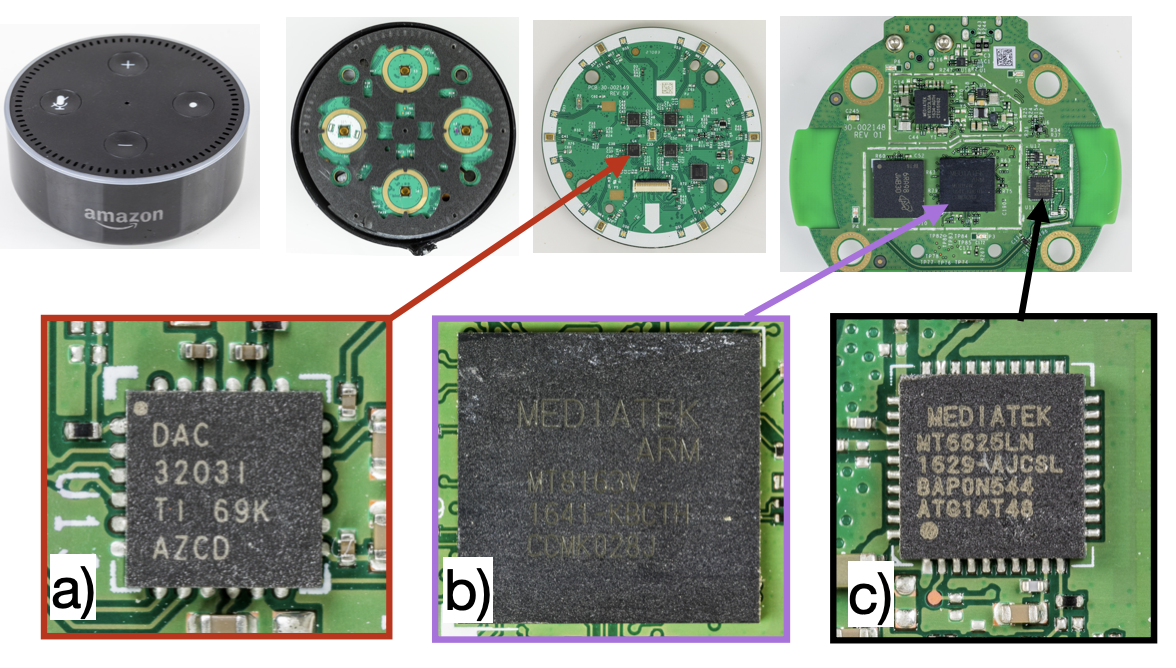
\includegraphics[width=\textwidth]{fig/echo-dot-inside}
\caption{Dissection de l'écho dot avec Zoom sur les composants étudiés. De G à D a) le convertisseur analog/digital de voix, b) le processeur et c) le chip MT6625LN avec les émetteurs/repcepeurs BT et wifi. Tiré de \cite{wikimedia-echo-dot}}
\label{fig:gain-var}
\end{center}
\end{figure}



%\textbf{Cours du 28/08}
%Système d'exploitation. Notion de priorité. Taper sur un clavier asynchorne 

%

%le Wifi peut avoir d'autres gamme de fréquences par ex. 5 GHz. Le wifi 1 Gps le BT 3 Mps \cite{wifi})
%\footnote{Chose que je ne savais pas le BT et le Wifi ont des fréquences identiques à 2.4 GHz, }

%A- priori Le Wifi peut avoir un débit de l'ordre de 1 Gps le BT en révanche 3 MBps. Chose que je ne savais pas l

%dans des maisons connectées  En tant que que futur enseignant d'informatique à l'heure ou le signal sans fil et l'internet des objets connait une énorme croissance fait partie intégrante et occupe une place grandissante dans notre notre quotidient. Ce sera le quotident des adultes de demains, à qui nous enseignons, avec la 5G  et les voitures autonome et les maisons connectées. es applications sont évidements énormes et ne font saisser de croitre. 
%les aspects.

%Comment sont-ils modulés et démodulés ?
%A quelles vitesse l'onde est elle échantillonnée? Quelles sont les limites de la quantié de donnée qui peut être transmises par secondes. 
%


%l'informationet le processeur de l'Echo dot une information est encodé sur une onde Wifi l'onde analogique qui contient l'information re-transmise dans la maison vers une ampoule qui elle aussi a un recepteur Wifi (cette information va donc être transformée en signal electrique qui allume la lumiére).
%Le signal numérique est transformé en onde radio

%les ondes porteuses sont conduits vers les antennes de réception, passe à travers le plastique et sont captés par le fil de cuivre de l'antenne. Ensuite ce signal est conduit vers la carte réseau du PC qui sert d'interface pour traduire les impulsions en données informatiques;

%Je

%et quels sont les developpement  de ces composants dans le but 

%Quelle est la différence fondamentales entre un signal Wifi et Bluetooth autre que la puissance et la quantité de données transmises, sont-ils échantillonés de la même façon?  : l'information doit être modulée ou démodulée d'une façon similaire pour les emmeteurs recepteurs BT et Wifi contenus sur la carte.



%Comment fonctionne en détail ce composant, comment l'information. Quels sont les débits. Y'at il d'autres différence que le débit entre le signal Wifi et BT (les deux sont à une fréquence de 2.4 GHz, le Wifi
%Comment l'information est elles modulé sur les ondes Wifi/BT.
%Quelle différence
%Quelle est la différence fondamentales entre un signal Wifi et bluetooth, sont-ils échantilloné de la même façon? L'onde wifi peut transmettre jusqu'à 1 Gps de données, le BT 3 Mps\cite{}.  Pourquoi choisir de communiquer avec la maison par Bluetooth plutot que Wifi?


%et le signal sans fil fera partie intégrante de leur quotidien. Pour pouvoir l'enseigner même à un niveau basique, il faut d'abord bien le comprendre.
%Débit de la transmission

 %Traitement numérique du signal.  Les deux signals ont la même fréquence centrée sur 2.4 GHz. Et plus généralement les aspects de traitement du signal Wifi/BT car les applications sont évidements énormes et ne font saisser de croitre. Directionalité versus Portée. On peut
%Transmission des données à 20 Gps pour la 5G. Comprendre les enjeux de transmissions de données avec la 5G. 2.4 GHz.
%D'une onde dans une gamme de fréquence donnée (anaéogique donc) à une information binaire.
%Wifi: 1 Gps
%4G: 1Gps
%BT: 3 Mps.
%Fréquence d'échantillonage

%\bibliographystyle{apalike}
\bibliographystyle{unsrt}
\bibliography{biblio}

\end{document}


